% Reproduction of Knobloch, Numer. Algorithms 94 (2023) 1229-1267, with galerkit.
% Tables and figures: galerkit examples/convection_diffusion/2d/kn23_reproduction/make_report.py --dest <this folder>
\documentclass[11pt]{article}

\usepackage[utf8]{inputenc}
\usepackage[T1]{fontenc}
\usepackage{lmodern}
\usepackage[margin=2.5cm]{geometry}
\usepackage{amsmath,amssymb,amsthm,mathtools}
\usepackage{enumitem}
\usepackage{booktabs}
\usepackage{xcolor}
\usepackage{graphicx}
\usepackage{url}
\usepackage{framed}
\usepackage[section]{placeins}
\usepackage[colorlinks=true,linkcolor=blue!60!black,citecolor=blue!60!black,urlcolor=blue!60!black]{hyperref}

\newcommand{\mism}[1]{\textcolor{orange!85!black}{#1}}
\newcommand{\eps}{\varepsilon}
\newcommand{\bb}{\boldsymbol{b}}
\newcommand{\R}{\mathbb{R}}
\newcommand{\yes}{\checkmark}

\title{The SMUAS method of Knobloch (Numer.\ Algorithms 2023):\\ implementation, algorithm, and numerical reproduction}
\author{galerkit}
\date{October 2026}

\begin{document}
\maketitle

\begin{abstract}
In \emph{An algebraically stabilized method for convection--diffusion--reaction problems with optimal experimental
convergence rates on general meshes}, P.~Knobloch studies why algebraic stabilizations can lose accuracy on meshes
without local symmetry and introduces the Symmetrized Monotone Upwind-type Algebraically Stabilized (SMUAS) method
\cite{Kn23}. This reproduction checks galerkit's implementations of all four methods considered in the paper—the AFC
schemes with the Kuzmin and BJK limiters, MUAS, and SMUAS—as well as the limiter variants used in the analysis. It
also presents SMUAS as an algorithm and recomputes the paper's numerical results: Tables~1--9, the statements in
Sections~5 and~6, and Figures~3, 4, 5, 7, 8, 9, 11, and~13. % generated by galerkit examples/convection_diffusion/2d/kn23_reproduction/make_report.py; do not edit
Of the 159 values of Tables~1--9 ($ne=16,\dots,512$, Table~5 up to $ne=256$; up to $5.3\cdot10^{5}$ unknowns), all agree with the paper in all printed digits.

\end{abstract}

\tableofcontents

%=====================================================================================================
\section{Is the method implemented?}\label{sec:impl}
%=====================================================================================================

\begin{table}[!htbp]
\renewcommand{\thetable}{I}
\centering\small\setlength{\tabcolsep}{4pt}
\caption{Methods and set-ups used in~\cite{Kn23} and their locations in galerkit
(\texttt{src/galerkit/convection\_diffusion}). Items marked ``new'' were added for this reproduction.}\label{tab:kn23-impl}
\begin{tabular}{p{6.2cm}p{8.6cm}}
\toprule
item of the paper & galerkit\\
\midrule
AFC, Kuzmin limiter (19)--(23), $R_i^\pm=1$ at Dirichlet nodes & \texttt{stab="afc\_kuzmin"} (limiter \texttt{"kuzmin"})\\
AFC, BJK limiter (25)--(28) with $a_{ji}:=0$ at Dirichlet nodes & \texttt{stab="afc"}, $\mu_i$ = \texttt{afc\_gamma} (a number, or \texttt{"bjk"} for (30))\\
MUAS (31)--(36) & \texttt{stab="muas"}\\
SMUAS (60)--(64) with (67) or (68) & \texttt{stab="smuas"}, \texttt{smuas\_weights="67"|"68"}\\
Kuzmin with $P_i^\pm$ from (25) (Fig.~7, right) & new: \texttt{AFCOperator(kuzmin\_p="25")}\\
$R_i^\pm=\min\{1,\mu_iQ_i^\pm/P_i^\pm\}$, (27), (47), (48) & new: \texttt{AFCOperator(r\_mu=}scalar or per node\texttt{)}\\
Example 1 & \texttt{bjk\_polynomial}\\
Examples 2--5 & new: \texttt{kn23\_ex2}, \dots, \texttt{kn23\_ex5} (Ex.~3 in an overflow-free form)\\
Grids 1, 4, 5; 6, 7, 8 & \texttt{rectangle\_mesh} (\texttt{right}, \texttt{rows}, \texttt{left}, \texttt{alternating}, \texttt{crossed}), \texttt{distorted\_rows\_mesh}\\
Grids 2, 3 & from the BJK16 reproduction (Grid~3 read from the vector figure of~\cite{BJK16})\\
Grid 9 & new: \texttt{kn23\_grids.grid9}\\
Table 9 grid (shift $1.5h$, last node $0.75h$) & new: \texttt{distorted\_rows\_mesh(last\_shift=0.75)}\\
Table 10: triangulated FVCA5 \texttt{mesh4\_1} family & \emph{not available} (see Section~\ref{sec:disc})\\
nonlinear solver ``fixed point rhs'' (Remark 5) & \texttt{afc\_solver="fp\_rhs"}; also \texttt{"newton"}, \texttt{"fp\_anderson"}\\
\bottomrule
\end{tabular}
\end{table}

\textbf{Answer: yes.} All four methods discussed in the paper were already implemented in galerkit. Tables~1, 2, 4,
the first row of Table~5, and Table~8 had also been checked previously. We verified the SMUAS implementation
(limiter \texttt{"smuas"} in\\ \texttt{src/galerkit/convection\_diffusion/afc.py}) line by line against
(61)--(68) of~\cite{Kn23}. In particular, the sums defining $P_i^\pm$ include only those $j\in S_i$ for which
$a_{ij}>0$ or $a_{ji}>0$, whereas the sums defining $Q_i^\pm$ include every $j\in S_i$. The reflected values are
$u_{ij}=u_i+\nabla u_h|_{T_{ij}}\cdot(x_i-x_j)$, where $T_{ij}$ is the simplex in the patch entered by the half-line
$x_i+t(x_i-x_j)$ for $t>0$. We also confirmed that $R_i^\pm=1$ at Dirichlet nodes and whenever $P_i^\pm=0$, and that
$\beta_{ij}$ and $b_{ij}$ are defined as in (36), (31), and (32). For this reproduction, we added the limiter
variants studied in Section~5 ($P_i^\pm$ from (25) for the Kuzmin limiter and the factor $\mu_i$ from (27)/(47) in
$R_i^\pm$), Examples~2--5, Grids~6--9, and the grid used for Table~9.

%=====================================================================================================
\section{The SMUAS algorithm}\label{sec:alg}
%=====================================================================================================

\paragraph{Setting.} We use $P_1$ elements on a simplicial triangulation of $\Omega\subset\R^d$. The nodes are
$x_1,\dots,x_N$, with $x_{M+1},\dots,x_N$ on $\partial\Omega$; $S_i$ denotes the neighbours of $x_i$, and $\Delta_i$
its patch. Let $A=(a_{ij})$ be the Galerkin matrix for $-\eps\Delta u+\bb\cdot\nabla u+cu=g$, with
$a_{ij}=a(\varphi_j,\varphi_i)$. The method seeks
\begin{equation}\label{eq:alg}
  \sum_{j=1}^N\bigl(a_{ij}+b_{ij}(U)\bigr)u_j=g_i,\quad i\le M,\qquad u_i=u_b(x_i),\quad i>M,
\end{equation}
where the symmetric stabilization matrix has zero row sums and is given by
$b_{ij}(U)=-\max\{\beta_{ij}(U)a_{ij},0,\beta_{ji}(U)a_{ji}\}$ ($i\ne j$), $b_{ii}=-\sum_{j\ne i}b_{ij}$.

\begin{framed}
\noindent\textbf{Algorithm SMUAS.}\quad\emph{Input:} $A$, $g$, $u_b$, the mesh, the choice (67) or (68) of the weights,
a tolerance $\tau$. \emph{Output:} $U$ solving \eqref{eq:alg}.

\smallskip\noindent\textbf{Set-up} (performed once for each mesh).
\begin{enumerate}[label=S\arabic*., leftmargin=*, itemsep=2pt]
\item For each interior node $i$ and each $j\in S_i$, find the simplex $T_{ij}\subset\Delta_i$ entered by the half
  line $\{x_i+t(x_i-x_j):t>0\}$. Equivalently, this is the simplex whose barycentric gradients satisfy
  $\nabla\lambda_k\cdot(x_i-x_j)\ge0$ for all its vertices $x_k\ne x_i$). Store the row
  $w_{ij}=e_i+\sum_{x_k\in T_{ij}}(\nabla\lambda_k\cdot(x_i-x_j))\,e_k$, so that the reflected value is
  $u_{ij}=w_{ij}\cdot U=u_i+\nabla u_h|_{T_{ij}}\cdot(x_i-x_j)$ \hfill(60)
\item Weights, (67): $p_{ij}=\max\{a_{ij},0,a_{ji}\}$, $q_{ij}=\max\{|a_{ij}|,a_{ji}\}$; or (68): $p_{ij}=q_{ij}=1$.
  Set $p_{ij}=0$ unless $a_{ij}>0$ or $a_{ji}>0$.
\end{enumerate}

\noindent\textbf{Stabilization matrix} $B(U)$ for a given iterate $U$.
\begin{enumerate}[label=B\arabic*., leftmargin=*, itemsep=2pt]
\item For $i\le M$ and $j\in S_i$: $\delta_{ij}=u_i-u_j$ and $r_{ij}=u_i-u_{ij}$.
\item $P_i^\pm=\sum_{j\in S_i}p_{ij}\{(\delta_{ij})^\pm+(r_{ij})^\pm\}$,\quad
  $Q_i^\pm=\sum_{j\in S_i}q_{ij}\{(-\delta_{ij})^\pm+(-r_{ij})^\pm\}$ \hfill(61)--(64)\\
  with $z^+=\max\{0,z\}$, $z^-=\min\{0,z\}$.
\item $R_i^\pm=\min\{1,Q_i^\pm/P_i^\pm\}$, and $R_i^\pm=1$ if $P_i^\pm=0$ or $i>M$. \hfill(20), (21)
\item $\beta_{ij}=1-R_i^+$ if $u_i>u_j$, $\beta_{ij}=1-R_i^-$ if $u_i<u_j$, $\beta_{ij}=0$ if $u_i=u_j$. \hfill(36)
\item $b_{ij}=-\max\{\beta_{ij}a_{ij},0,\beta_{ji}a_{ji}\}$ for every edge, $b_{ii}=-\sum_{j\neq i}b_{ij}$. \hfill(31), (32)
\end{enumerate}

\noindent\textbf{Nonlinear solve.} Let $D$ denote the matrix obtained from $B$ by setting all $\beta_{ij}=1$;
thus, $d_{ij}=-\max\{a_{ij},0,a_{ji}\}$.
\begin{enumerate}[label=N\arabic*., leftmargin=*, itemsep=2pt]
\item Find the monotone low-order solution $U^0$ by solving $(A+D)U^0=g$ with the prescribed Dirichlet values.
\item For $k=0,1,\dots$: compute $B(U^k)$ by B1--B5 and the residual
  $r^k=g-(A+B(U^k))U^k$ on the free nodes; stop if $\|r^k\|_2\le\tau$.
\item \emph{Fixed point rhs} (used in~\cite{Kn23}, Remark~5): solve
  $(A+D)\tilde U=g-(B(U^k)-D)U^k$ using the factorization of $A+D$ computed in N1, then set
  $U^{k+1}=U^k+\omega_k(\tilde U-U^k)$ with damping parameter $\omega_k\in(0,1]$; or
  \emph{semismooth Newton}: $U^{k+1}=U^k-\lambda_k J(U^k)^{-1}r^k$ with the generalized Jacobian of the piecewise
  smooth map $U\mapsto(A+B(U))U$ and an Armijo step $\lambda_k$.
\end{enumerate}
\end{framed}

\paragraph{Properties.} For arbitrary simplicial meshes,~\cite{Kn23} proves (A1), and thus the existence of a
solution (Theorem~4), as well as the local DMP via (A2) (Theorem~5) and linearity preservation (Remark~2). In
particular, for $u_h\in P_1(\R^d)$, $r_{ij}=-\delta_{ij}$, and therefore
$P_i^+=-P_i^-=\sum_j p_{ij}|u_i-u_j|\le\sum_j q_{ij}|u_i-u_j|=Q_i^+=-Q_i^-$ by $p_{ij}\le q_{ij}$, so $R_i^\pm=1$ and
$B(U)=0$).
Each evaluation of $B(U)$ requires one sparse matrix-vector product $WU$ to compute the reflected values, followed
by loops over the edges. Its cost is therefore linear in the number of edges. The set-up step S1 requires just one
pass over the patches.

\paragraph{Implementation in galerkit.}
\begin{itemize}[leftmargin=*, itemsep=1pt]
\item S1: \texttt{reflection\_operator}, a sparse matrix $W$ with one row per directed edge;
\item B1--B5: \texttt{AFCOperator.b\_edges};
\item N1--N3: \texttt{solve\_afc} with \texttt{afc\_solver} set to \texttt{"fp\_rhs"}, \texttt{"fp\_anderson"}
  (Anderson acceleration) or \texttt{"newton"} (exact generalized Jacobian of SMUAS, \texttt{\_jacobian\_muas}).
\end{itemize}

%=====================================================================================================
\section{Set-up of the computations}\label{sec:setup}
%=====================================================================================================

\begin{itemize}[leftmargin=*]
\item We use $P_1$ elements and do not lump the reaction term, unlike~\cite{BJK16}. The values of $\varepsilon$ are
  as specified for each example.
\item We define $ne$ as the number of edges along the part of $\partial\Omega$ where $y=1$. Grids~1 and~4--8 have
  $ne\times ne$ squares. Grid~2 starts with $ne=2$ and Grid~3 with $ne=4$ on level~0; both are then uniformly
  refined, giving grids with the same $ne$ similar numbers of triangles. Grid~9 is generated separately for each
  value of $ne$.
\item We compute the error norm
  $\|v\|_h^2=\varepsilon|v|_1^2+\sigma_0\|v\|_0^2+b_h(u_h;v,v)$ for $v=u-u_h$, evaluating the last term at
  $i_hu-u_h$, and set $\sigma_0=1$. For Example~2, where $c=0$, Table~3 is reproduced only with $\sigma_0=1$; that
  is, we retain the $L^2$ term even though the paper sets $\sigma_0=0$. For $ne=16$, omitting it gives
  $\sqrt{\varepsilon|e|_1^2+b_h}=8.560\cdot10^{-3}$, whereas the printed value is
  $1.179\cdot10^{-2}=\sqrt{(8.560\cdot10^{-3})^2+\|e\|_0^2}$.
\item We use semismooth Newton with the exact generalized Jacobian for Kuzmin, MUAS, and SMUAS, and coloured finite
  differences for the variants. Iterations stop when the Euclidean residual reaches $10^{-10}$. When Newton is
  slow, we use the Anderson-accelerated fixed point rhs method. Although the paper uses fixed point rhs, the results
  are solver-independent once the residual is sufficiently small.
\item We interpret ``odd horizontal grid lines'' in (47) and (48) as lines counted from $y=0$, with the first line
  indexed by~1; thus, the selected lines are $y=0,2h,4h,\dots$. With $\mu$ on these lines, Example~2 is solved
  exactly; placing $\mu$ on the other lines gives an error of $2.5\cdot10^{-2}$.
\end{itemize}

%=====================================================================================================
\section{Tables}\label{sec:tables}
%=====================================================================================================

% generated by galerkit examples/convection_diffusion/2d/kn23_reproduction/make_report.py; do not edit
\begin{table}[!htbp]
\renewcommand{\thetable}{S}
\centering\small\setlength{\tabcolsep}{4pt}
\caption{Agreement with Tables~1--9 of~\cite{Kn23}: entries computed, entries differing in the printed digits, largest relative deviation from the printed values (the printing rounds by up to $5\cdot10^{-4}$), and the largest final Euclidean residual of the nonlinear solve.}\label{tab:kn23-summary}
\begin{tabular}{rp{8.2cm}crrrr}
\toprule
Table & case & $ne$ & entries & differ & max dev. & residual\\
\midrule
1 & Example 1, $\varepsilon=10^{-8}$, Grid 1, AFC with the Kuzmin limiter & 16--512 & 18 & 0 & 3.2e-04 & 6e-14 \\
2 & Example 1, $\varepsilon=10^{-8}$, Grid 4, AFC with the Kuzmin limiter & 16--512 & 18 & 0 & 3.1e-04 & 1e-10 \\
3 & Example 2, Grid 4, AFC with the Kuzmin limiter & 16--512 & 18 & 0 & 3.7e-04 & 1e-10 \\
4 & Example 1, $\varepsilon=10^{-8}$, Grid 4, SMUAS with (67) & 16--512 & 18 & 0 & 3.0e-04 & 9e-11 \\
5 & Example 1, $\varepsilon=10^{-8}$, Grid 4, SMUAS with (68) & 16--256 & 15 & 0 & 4.6e-04 & 1e-12 \\
6 & Example 1, $\varepsilon=10^{-8}$, Grid 2, SMUAS with (67) & 16--512 & 18 & 0 & 3.7e-04 & 2e-11 \\
7 & Example 1, $\varepsilon=10^{-8}$, Grid 3, SMUAS with (68) & 16--512 & 18 & 0 & 3.4e-04 & 3e-11 \\
8 & Example 1, $\varepsilon=10$, Grid 5 with shift $0.8h$, SMUAS with (67) & 16--512 & 18 & 0 & 4.3e-04 & 1e-12 \\
9 & Example 1, $\varepsilon=10$, Grid 5 with shift $1.5h$ ($0.75h$ for the last node), SMUAS with (67) & 16--512 & 18 & 0 & 2.8e-04 & 7e-11 \\
\bottomrule
\end{tabular}
\end{table}

% generated by galerkit examples/convection_diffusion/2d/kn23_reproduction/make_report.py; do not edit
\setcounter{table}{0}
\begin{table}[!htbp]
\centering\small\setlength{\tabcolsep}{4pt}
\caption{Example 1, $\varepsilon=10^{-8}$, Grid 1, AFC with the Kuzmin limiter. galerkit values; ``ord.'' is $\log_2$ of the ratio to the previous row. Every entry agrees with the paper in all printed digits.}\label{tab:kn23-t1}
\begin{tabular}{r rr rr rr}
\toprule
$ne$ & $\|u-u_h\|_{0}$ & ord. & $|u-u_h|_{1}$ & ord. & $\|u-u_h\|_h$ & ord.\\
\midrule
16 & $1.934\mathrm{e}{-2}$ &  & $4.937\mathrm{e}{-1}$ &  & $5.007\mathrm{e}{-2}$ &  \\
32 & $5.359\mathrm{e}{-3}$ & 1.85 & $2.305\mathrm{e}{-1}$ & 1.10 & $1.149\mathrm{e}{-2}$ & 2.12 \\
64 & $1.385\mathrm{e}{-3}$ & 1.95 & $1.082\mathrm{e}{-1}$ & 1.09 & $2.649\mathrm{e}{-3}$ & 2.12 \\
128 & $3.442\mathrm{e}{-4}$ & 2.01 & $5.154\mathrm{e}{-2}$ & 1.07 & $6.152\mathrm{e}{-4}$ & 2.11 \\
256 & $8.536\mathrm{e}{-5}$ & 2.01 & $2.566\mathrm{e}{-2}$ & 1.01 & $1.586\mathrm{e}{-4}$ & 1.96 \\
512 & $2.126\mathrm{e}{-5}$ & 2.01 & $1.342\mathrm{e}{-2}$ & 0.93 & $3.876\mathrm{e}{-5}$ & 2.03 \\
\bottomrule
\end{tabular}
\end{table}

\setcounter{table}{1}
\begin{table}[!htbp]
\centering\small\setlength{\tabcolsep}{4pt}
\caption{Example 1, $\varepsilon=10^{-8}$, Grid 4, AFC with the Kuzmin limiter. galerkit values; ``ord.'' is $\log_2$ of the ratio to the previous row. Every entry agrees with the paper in all printed digits.}\label{tab:kn23-t2}
\begin{tabular}{r rr rr rr}
\toprule
$ne$ & $\|u-u_h\|_{0}$ & ord. & $|u-u_h|_{1}$ & ord. & $\|u-u_h\|_h$ & ord.\\
\midrule
16 & $2.019\mathrm{e}{-2}$ &  & $6.005\mathrm{e}{-1}$ &  & $5.663\mathrm{e}{-2}$ &  \\
32 & $6.285\mathrm{e}{-3}$ & 1.68 & $4.832\mathrm{e}{-1}$ & 0.31 & $2.138\mathrm{e}{-2}$ & 1.41 \\
64 & $2.308\mathrm{e}{-3}$ & 1.45 & $4.549\mathrm{e}{-1}$ & 0.09 & $9.485\mathrm{e}{-3}$ & 1.17 \\
128 & $1.092\mathrm{e}{-3}$ & 1.08 & $4.442\mathrm{e}{-1}$ & 0.03 & $4.490\mathrm{e}{-3}$ & 1.08 \\
256 & $5.543\mathrm{e}{-4}$ & 0.98 & $4.368\mathrm{e}{-1}$ & 0.02 & $2.187\mathrm{e}{-3}$ & 1.04 \\
512 & $2.823\mathrm{e}{-4}$ & 0.97 & $4.327\mathrm{e}{-1}$ & 0.01 & $1.083\mathrm{e}{-3}$ & 1.01 \\
\bottomrule
\end{tabular}
\end{table}

\setcounter{table}{2}
\begin{table}[!htbp]
\centering\small\setlength{\tabcolsep}{4pt}
\caption{Example 2, Grid 4, AFC with the Kuzmin limiter. galerkit values; ``ord.'' is $\log_2$ of the ratio to the previous row. Every entry agrees with the paper in all printed digits.}\label{tab:kn23-t3}
\begin{tabular}{r rr rr rr}
\toprule
$ne$ & $\|u-u_h\|_{0}$ & ord. & $|u-u_h|_{1}$ & ord. & $\|u-u_h\|_h$ & ord.\\
\midrule
16 & $8.104\mathrm{e}{-3}$ &  & $4.401\mathrm{e}{-1}$ &  & $1.179\mathrm{e}{-2}$ &  \\
32 & $4.291\mathrm{e}{-3}$ & 0.92 & $4.700\mathrm{e}{-1}$ & -0.09 & $6.227\mathrm{e}{-3}$ & 0.92 \\
64 & $2.204\mathrm{e}{-3}$ & 0.96 & $4.851\mathrm{e}{-1}$ & -0.05 & $3.157\mathrm{e}{-3}$ & 0.98 \\
128 & $1.117\mathrm{e}{-3}$ & 0.98 & $4.926\mathrm{e}{-1}$ & -0.02 & $1.580\mathrm{e}{-3}$ & 1.00 \\
256 & $5.618\mathrm{e}{-4}$ & 0.99 & $4.963\mathrm{e}{-1}$ & -0.01 & $7.893\mathrm{e}{-4}$ & 1.00 \\
512 & $2.817\mathrm{e}{-4}$ & 1.00 & $4.982\mathrm{e}{-1}$ & -0.01 & $3.974\mathrm{e}{-4}$ & 0.99 \\
\bottomrule
\end{tabular}
\end{table}

\setcounter{table}{3}
\begin{table}[!htbp]
\centering\small\setlength{\tabcolsep}{4pt}
\caption{Example 1, $\varepsilon=10^{-8}$, Grid 4, SMUAS with (67). galerkit values; ``ord.'' is $\log_2$ of the ratio to the previous row. Every entry agrees with the paper in all printed digits.}\label{tab:kn23-t4}
\begin{tabular}{r rr rr rr}
\toprule
$ne$ & $\|u-u_h\|_{0}$ & ord. & $|u-u_h|_{1}$ & ord. & $\|u-u_h\|_h$ & ord.\\
\midrule
16 & $2.147\mathrm{e}{-2}$ &  & $4.734\mathrm{e}{-1}$ &  & $5.530\mathrm{e}{-2}$ &  \\
32 & $6.353\mathrm{e}{-3}$ & 1.76 & $2.529\mathrm{e}{-1}$ & 0.90 & $1.479\mathrm{e}{-2}$ & 1.90 \\
64 & $1.783\mathrm{e}{-3}$ & 1.83 & $1.363\mathrm{e}{-1}$ & 0.89 & $3.922\mathrm{e}{-3}$ & 1.92 \\
128 & $4.706\mathrm{e}{-4}$ & 1.92 & $7.220\mathrm{e}{-2}$ & 0.92 & $1.054\mathrm{e}{-3}$ & 1.90 \\
256 & $1.221\mathrm{e}{-4}$ & 1.95 & $3.807\mathrm{e}{-2}$ & 0.92 & $2.940\mathrm{e}{-4}$ & 1.84 \\
512 & $3.135\mathrm{e}{-5}$ & 1.96 & $2.002\mathrm{e}{-2}$ & 0.93 & $7.896\mathrm{e}{-5}$ & 1.90 \\
\bottomrule
\end{tabular}
\end{table}

\setcounter{table}{4}
\begin{table}[!htbp]
\centering\small\setlength{\tabcolsep}{4pt}
\caption{Example 1, $\varepsilon=10^{-8}$, Grid 4, SMUAS with (68). galerkit values; ``ord.'' is $\log_2$ of the ratio to the previous row. Every entry agrees with the paper in all printed digits.}\label{tab:kn23-t5}
\begin{tabular}{r rr rr rr}
\toprule
$ne$ & $\|u-u_h\|_{0}$ & ord. & $|u-u_h|_{1}$ & ord. & $\|u-u_h\|_h$ & ord.\\
\midrule
16 & $2.208\mathrm{e}{-2}$ &  & $4.748\mathrm{e}{-1}$ &  & $5.702\mathrm{e}{-2}$ &  \\
32 & $6.605\mathrm{e}{-3}$ & 1.74 & $2.515\mathrm{e}{-1}$ & 0.92 & $1.530\mathrm{e}{-2}$ & 1.90 \\
64 & $1.860\mathrm{e}{-3}$ & 1.83 & $1.336\mathrm{e}{-1}$ & 0.91 & $4.008\mathrm{e}{-3}$ & 1.93 \\
128 & $4.924\mathrm{e}{-4}$ & 1.92 & $6.959\mathrm{e}{-2}$ & 0.94 & $1.046\mathrm{e}{-3}$ & 1.94 \\
256 & $1.279\mathrm{e}{-4}$ & 1.95 & $3.635\mathrm{e}{-2}$ & 0.94 & $2.823\mathrm{e}{-4}$ & 1.89 \\
\bottomrule
\end{tabular}
\end{table}

\setcounter{table}{5}
\begin{table}[!htbp]
\centering\small\setlength{\tabcolsep}{4pt}
\caption{Example 1, $\varepsilon=10^{-8}$, Grid 2, SMUAS with (67). galerkit values; ``ord.'' is $\log_2$ of the ratio to the previous row. Every entry agrees with the paper in all printed digits.}\label{tab:kn23-t6}
\begin{tabular}{r rr rr rr}
\toprule
$ne$ & $\|u-u_h\|_{0}$ & ord. & $|u-u_h|_{1}$ & ord. & $\|u-u_h\|_h$ & ord.\\
\midrule
16 & $9.950\mathrm{e}{-3}$ &  & $2.432\mathrm{e}{-1}$ &  & $1.956\mathrm{e}{-2}$ &  \\
32 & $2.764\mathrm{e}{-3}$ & 1.85 & $1.125\mathrm{e}{-1}$ & 1.11 & $4.638\mathrm{e}{-3}$ & 2.08 \\
64 & $7.357\mathrm{e}{-4}$ & 1.91 & $5.210\mathrm{e}{-2}$ & 1.11 & $1.139\mathrm{e}{-3}$ & 2.03 \\
128 & $1.889\mathrm{e}{-4}$ & 1.96 & $2.461\mathrm{e}{-2}$ & 1.08 & $2.812\mathrm{e}{-4}$ & 2.02 \\
256 & $4.778\mathrm{e}{-5}$ & 1.98 & $1.189\mathrm{e}{-2}$ & 1.05 & $6.888\mathrm{e}{-5}$ & 2.03 \\
512 & $1.202\mathrm{e}{-5}$ & 1.99 & $5.837\mathrm{e}{-3}$ & 1.03 & $1.709\mathrm{e}{-5}$ & 2.01 \\
\bottomrule
\end{tabular}
\end{table}

\setcounter{table}{6}
\begin{table}[!htbp]
\centering\small\setlength{\tabcolsep}{4pt}
\caption{Example 1, $\varepsilon=10^{-8}$, Grid 3, SMUAS with (68). galerkit values; ``ord.'' is $\log_2$ of the ratio to the previous row. Every entry agrees with the paper in all printed digits.}\label{tab:kn23-t7}
\begin{tabular}{r rr rr rr}
\toprule
$ne$ & $\|u-u_h\|_{0}$ & ord. & $|u-u_h|_{1}$ & ord. & $\|u-u_h\|_h$ & ord.\\
\midrule
16 & $2.218\mathrm{e}{-2}$ &  & $4.338\mathrm{e}{-1}$ &  & $5.994\mathrm{e}{-2}$ &  \\
32 & $7.257\mathrm{e}{-3}$ & 1.61 & $2.175\mathrm{e}{-1}$ & 1.00 & $1.637\mathrm{e}{-2}$ & 1.87 \\
64 & $2.093\mathrm{e}{-3}$ & 1.79 & $1.009\mathrm{e}{-1}$ & 1.11 & $4.066\mathrm{e}{-3}$ & 2.01 \\
128 & $5.703\mathrm{e}{-4}$ & 1.88 & $4.635\mathrm{e}{-2}$ & 1.12 & $1.000\mathrm{e}{-3}$ & 2.02 \\
256 & $1.520\mathrm{e}{-4}$ & 1.91 & $2.184\mathrm{e}{-2}$ & 1.09 & $2.524\mathrm{e}{-4}$ & 1.99 \\
512 & $4.046\mathrm{e}{-5}$ & 1.91 & $1.046\mathrm{e}{-2}$ & 1.06 & $6.448\mathrm{e}{-5}$ & 1.97 \\
\bottomrule
\end{tabular}
\end{table}

\setcounter{table}{7}
\begin{table}[!htbp]
\centering\small\setlength{\tabcolsep}{4pt}
\caption{Example 1, $\varepsilon=10$, Grid 5 with shift $0.8h$, SMUAS with (67). galerkit values; ``ord.'' is $\log_2$ of the ratio to the previous row. Every entry agrees with the paper in all printed digits.}\label{tab:kn23-t8}
\begin{tabular}{r rr rr rr}
\toprule
$ne$ & $\|u-u_h\|_{0}$ & ord. & $|u-u_h|_{1}$ & ord. & $\|u-u_h\|_h$ & ord.\\
\midrule
16 & $3.155\mathrm{e}{-2}$ &  & $5.855\mathrm{e}{-1}$ &  & $1.976\mathrm{e}{0}$ &  \\
32 & $7.267\mathrm{e}{-3}$ & 2.12 & $3.002\mathrm{e}{-1}$ & 0.96 & $9.676\mathrm{e}{-1}$ & 1.03 \\
64 & $1.665\mathrm{e}{-3}$ & 2.13 & $1.518\mathrm{e}{-1}$ & 0.98 & $4.826\mathrm{e}{-1}$ & 1.00 \\
128 & $4.111\mathrm{e}{-4}$ & 2.02 & $7.642\mathrm{e}{-2}$ & 0.99 & $2.420\mathrm{e}{-1}$ & 1.00 \\
256 & $1.048\mathrm{e}{-4}$ & 1.97 & $3.837\mathrm{e}{-2}$ & 0.99 & $1.214\mathrm{e}{-1}$ & 1.00 \\
512 & $2.659\mathrm{e}{-5}$ & 1.98 & $1.922\mathrm{e}{-2}$ & 1.00 & $6.080\mathrm{e}{-2}$ & 1.00 \\
\bottomrule
\end{tabular}
\end{table}

\setcounter{table}{8}
\begin{table}[!htbp]
\centering\small\setlength{\tabcolsep}{4pt}
\caption{Example 1, $\varepsilon=10$, Grid 5 with shift $1.5h$ ($0.75h$ for the last node), SMUAS with (67). galerkit values; ``ord.'' is $\log_2$ of the ratio to the previous row. Every entry agrees with the paper in all printed digits.}\label{tab:kn23-t9}
\begin{tabular}{r rr rr rr}
\toprule
$ne$ & $\|u-u_h\|_{0}$ & ord. & $|u-u_h|_{1}$ & ord. & $\|u-u_h\|_h$ & ord.\\
\midrule
16 & $7.338\mathrm{e}{-2}$ &  & $8.767\mathrm{e}{-1}$ &  & $3.620\mathrm{e}{0}$ &  \\
32 & $2.287\mathrm{e}{-2}$ & 1.68 & $4.854\mathrm{e}{-1}$ & 0.85 & $1.732\mathrm{e}{0}$ & 1.06 \\
64 & $5.395\mathrm{e}{-3}$ & 2.08 & $2.506\mathrm{e}{-1}$ & 0.95 & $8.234\mathrm{e}{-1}$ & 1.07 \\
128 & $1.319\mathrm{e}{-3}$ & 2.03 & $1.281\mathrm{e}{-1}$ & 0.97 & $4.091\mathrm{e}{-1}$ & 1.01 \\
256 & $3.541\mathrm{e}{-4}$ & 1.90 & $6.501\mathrm{e}{-2}$ & 0.98 & $2.062\mathrm{e}{-1}$ & 0.99 \\
512 & $9.619\mathrm{e}{-5}$ & 1.88 & $3.275\mathrm{e}{-2}$ & 0.99 & $1.037\mathrm{e}{-1}$ & 0.99 \\
\bottomrule
\end{tabular}
\end{table}


%=====================================================================================================
\section{The statements of Sections 5 and 6}\label{sec:checks}
%=====================================================================================================

% generated by galerkit examples/convection_diffusion/2d/kn23_reproduction/make_report.py; do not edit
\begin{table}[!htbp]
\renewcommand{\thetable}{C1}
\centering\small
\caption{Example~2, AFC with the Kuzmin limiter on Grid~4: in the interior, $u_h=x+\alpha$ on the odd and $u_h=x-\beta$ on the even horizontal grid lines, (40), (41); $\alpha$, $\beta$ are medians over $[0.2,0.8]^2$. $\alpha+\beta$ against $\delta$ of (46), and the maximal nodal error.}\label{tab:kn23-c1}
\begin{tabular}{rrrrrr}
\toprule
$ne$ & $\alpha$ & $\beta$ & $\alpha+\beta$ & $\delta=h^2/(2h-3\varepsilon)$ & $\max|u_h-u|$\\
\midrule
20 & 1.2004e-02 & 1.2947e-02 & 2.4952e-02 & 2.5000e-02 & 1.532e-02 \\
40 & 6.0052e-03 & 6.4946e-03 & 1.2500e-02 & 1.2500e-02 & 7.717e-03 \\
80 & 3.0026e-03 & 3.2473e-03 & 6.2500e-03 & 6.2500e-03 & 3.879e-03 \\
\bottomrule
\end{tabular}
\end{table}

\begin{itemize}[leftmargin=*]
\item Example~2 with the Kuzmin limiter modified by (47), (48) on the odd lines (Grid~4, $ne=20$): maximal nodal error 3.2e-08 (final residual 1e-10), i.e.\ the exact solution is recovered, as stated in Section~5.
\item SMUAS with (67) on Example~2: maximal nodal errors on Grids 1--9 ($ne=16$): 7e-16 1e-08 2e-08 2e-12 7e-14 7e-16 1e-15 2e-15 1e-08; the method is exact on every grid (the larger values are the tolerance of the nonlinear solve).
\item Example~3, Kuzmin on Grid~1 ($ne=20$): nodal error 9e-14 except on the last interior vertical line, where it is 0.029 (Fig.~7, left).
\item Example~3, SMUAS on Grid~4 ($ne=20$): with (68) the nodal error is below $10^{-9}$ except on the last interior vertical line, as stated in Section~6. With (67) the solution has an error of 1.1e-03 also on the second-last line.
\end{itemize}

\begin{table}[!htbp]
\renewcommand{\thetable}{C2}
\centering\small\setlength{\tabcolsep}{4pt}
\caption{Example~5: the convergence statements of Sections~5 and~6 (no table in the paper).}\label{tab:kn23-c2}
\begin{tabular}{lrrrrrrr}
\toprule
method & $ne$ & $\|e\|_0$ & $|e|_1$ & $\|e\|_h$ & \multicolumn{3}{c}{orders}\\
\midrule
Kuzmin, Grid 1 & 16 & $3.299\mathrm{e}{-4}$ & $3.724\mathrm{e}{-2}$ & $3.299\mathrm{e}{-4}$ &  &  &  \\
 & 32 & $8.247\mathrm{e}{-5}$ & $1.862\mathrm{e}{-2}$ & $8.249\mathrm{e}{-5}$ & 2.00 & 1.00 & 2.00 \\
 & 64 & $2.062\mathrm{e}{-5}$ & $9.307\mathrm{e}{-3}$ & $2.064\mathrm{e}{-5}$ & 2.00 & 1.00 & 2.00 \\
 & 128 & $5.156\mathrm{e}{-6}$ & $4.653\mathrm{e}{-3}$ & $5.177\mathrm{e}{-6}$ & 2.00 & 1.00 & 2.00 \\
\addlinespace
Kuzmin, Grid 4 & 16 & $2.310\mathrm{e}{-2}$ & $8.354\mathrm{e}{-1}$ & $3.454\mathrm{e}{-2}$ &  &  &  \\
 & 32 & $1.169\mathrm{e}{-2}$ & $8.277\mathrm{e}{-1}$ & $1.826\mathrm{e}{-2}$ & 0.98 & 0.01 & 0.92 \\
 & 64 & $5.893\mathrm{e}{-3}$ & $8.255\mathrm{e}{-1}$ & $9.434\mathrm{e}{-3}$ & 0.99 & 0.00 & 0.95 \\
 & 128 & $2.960\mathrm{e}{-3}$ & $8.246\mathrm{e}{-1}$ & $4.798\mathrm{e}{-3}$ & 0.99 & 0.00 & 0.98 \\
\addlinespace
SMUAS (67), Grid 4 & 16 & $1.617\mathrm{e}{-3}$ & $5.646\mathrm{e}{-2}$ & $1.827\mathrm{e}{-3}$ &  &  &  \\
 & 32 & $4.130\mathrm{e}{-4}$ & $2.684\mathrm{e}{-2}$ & $4.705\mathrm{e}{-4}$ & 1.97 & 1.07 & 1.96 \\
 & 64 & $1.042\mathrm{e}{-4}$ & $1.292\mathrm{e}{-2}$ & $1.186\mathrm{e}{-4}$ & 1.99 & 1.05 & 1.99 \\
 & 128 & $2.616\mathrm{e}{-5}$ & $6.313\mathrm{e}{-3}$ & $2.972\mathrm{e}{-5}$ & 1.99 & 1.03 & 2.00 \\
\bottomrule
\end{tabular}
\end{table}


%=====================================================================================================
\section{Figures}\label{sec:figs}
%=====================================================================================================

As in the paper, the figures show wire-frame plots of $u_h$ along grid lines parallel to the coordinate axes. They
are intended as qualitative comparisons and agree with the paper on every feature it describes.

\begin{figure}[!htbp]\centering
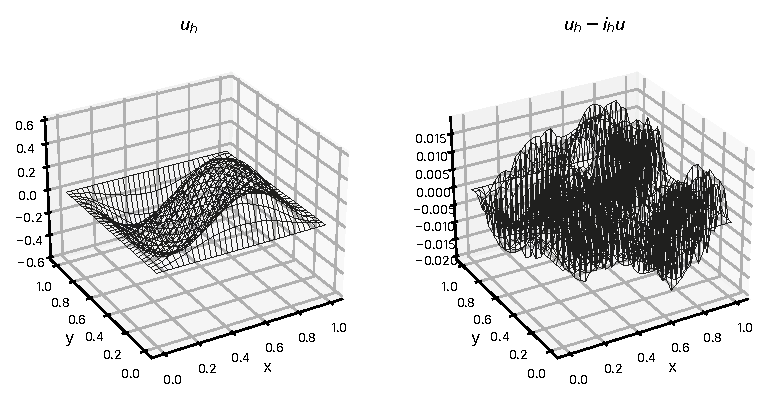
\includegraphics[width=0.75\textwidth]{figures/kn23_fig3.pdf}
\caption{(Fig.~3 of~\cite{Kn23}) Example~1, $\varepsilon=10^{-8}$, Kuzmin, Grid~4, $ne=32$: $u_h$ and $u_h-i_hu$.}\end{figure}
\begin{figure}[!htbp]\centering
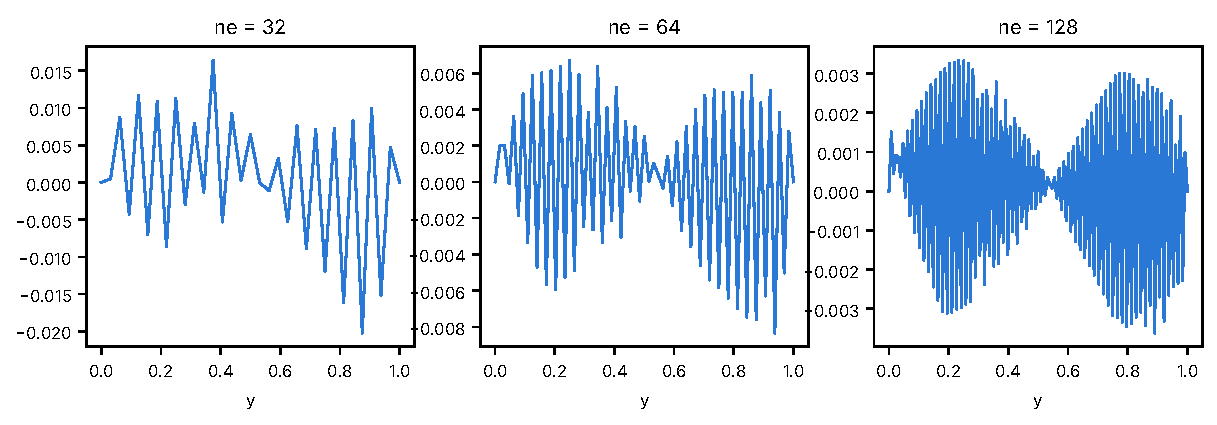
\includegraphics[width=\textwidth]{figures/kn23_fig4.pdf}
\caption{(Fig.~4) $u_h-i_hu$ along $x=0.25$ for $ne=32,64,128$. The amplitudes ($\approx0.02$, $0.007$, and $0.003$)
are consistent with the vertical scales in the paper.}\end{figure}
\begin{figure}[!htbp]\centering
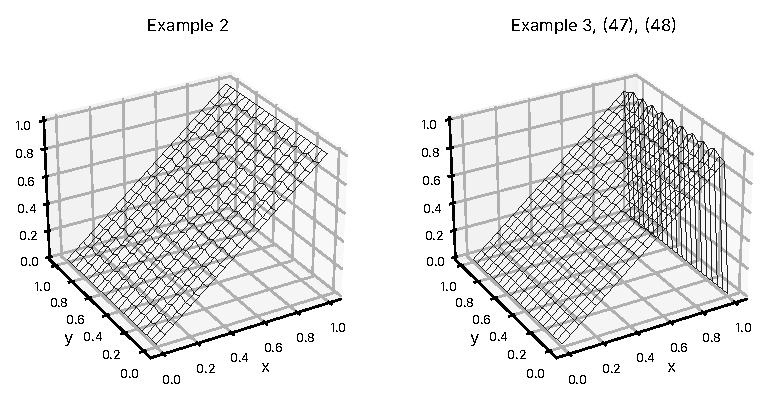
\includegraphics[width=0.75\textwidth]{figures/kn23_fig5.pdf}
\caption{(Fig.~5) Kuzmin, Grid~4, $ne=20$: Example~2, and Example~3 with (47), (48).}\end{figure}
\begin{figure}[!htbp]\centering
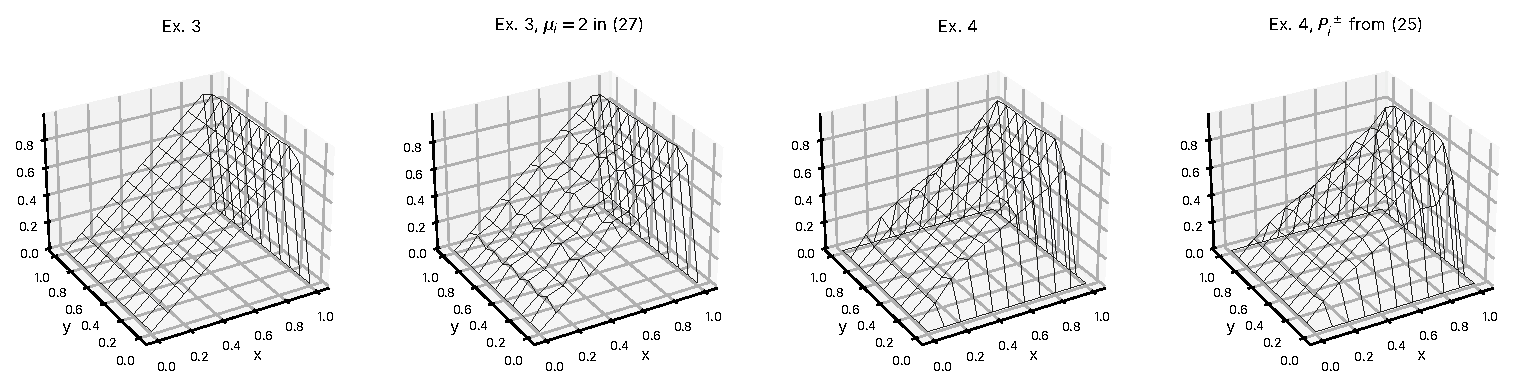
\includegraphics[width=\textwidth]{figures/kn23_fig7.pdf}
\caption{(Fig.~7) Kuzmin, Grid~1, $ne=10$: Example~3; Example~3 with $\mu_i=2$ in (27); Example~4; Example~4 with
$P_i^\pm$ from (25).}\end{figure}
\begin{figure}[!htbp]\centering
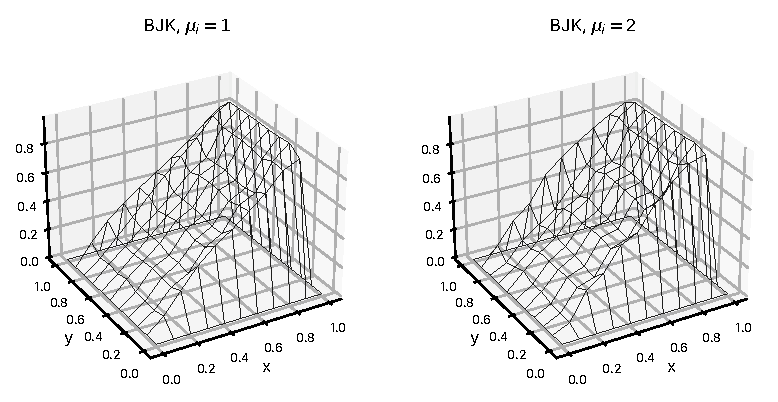
\includegraphics[width=0.75\textwidth]{figures/kn23_fig8.pdf}
\caption{(Fig.~8) Example~4, BJK limiter, Grid~1, $ne=10$, $\mu_i=1$ and $\mu_i=2$.}\end{figure}
\begin{figure}[!htbp]\centering
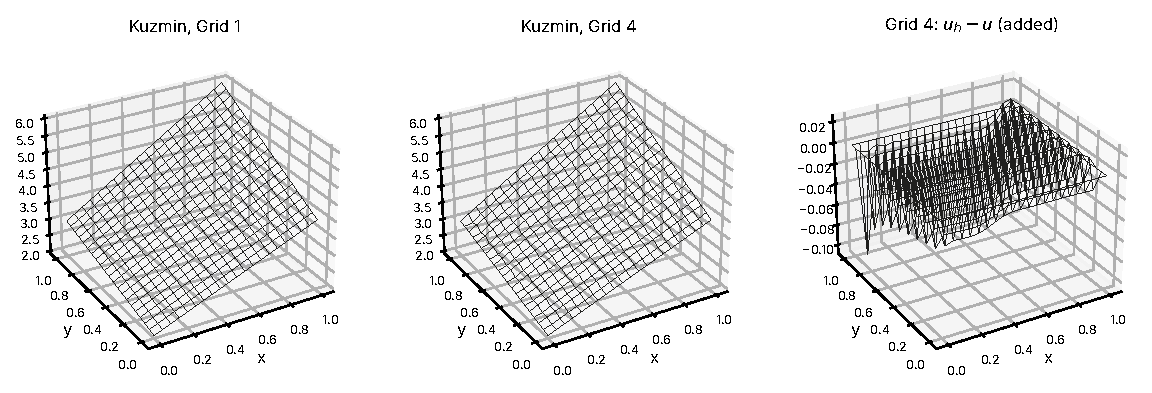
\includegraphics[width=\textwidth]{figures/kn23_fig9.pdf}
\caption{(Fig.~9) Example~5 with the Kuzmin limiter on Grids~1 and~4 for $ne=20$. The third panel, added here,
shows $u_h-u$ on Grid~4, where the oscillation is easier to see than in the solution itself.}\end{figure}
\begin{figure}[!htbp]\centering
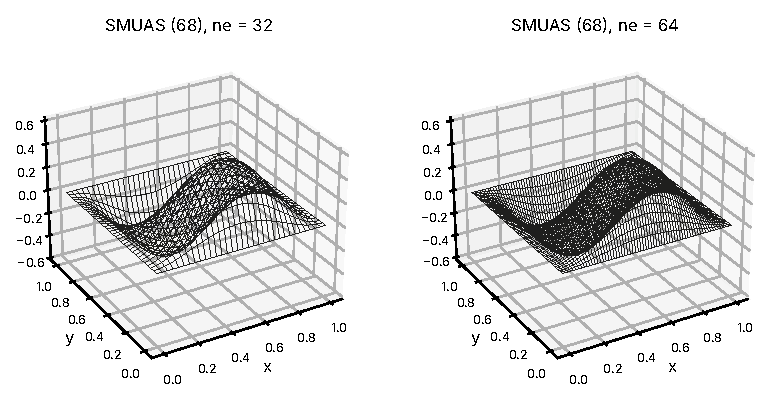
\includegraphics[width=0.75\textwidth]{figures/kn23_fig11.pdf}
\caption{(Fig.~11) Example~1, $\varepsilon=10^{-8}$, SMUAS (68), Grid~4, $ne=32$ and $64$; compare Fig.~3.}\end{figure}
\begin{figure}[!htbp]\centering
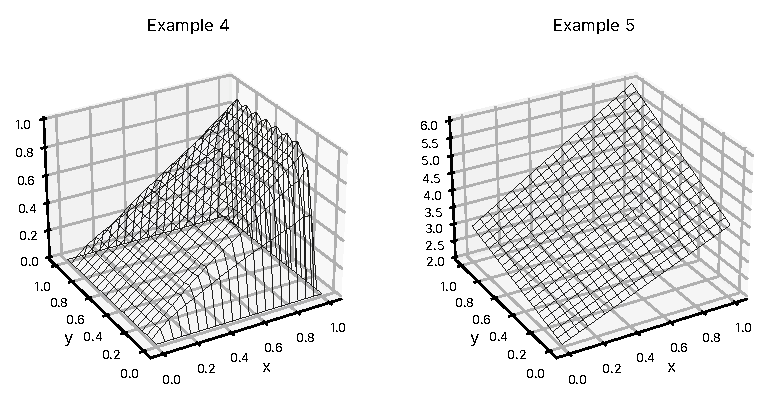
\includegraphics[width=0.75\textwidth]{figures/kn23_fig13.pdf}
\caption{(Fig.~13) SMUAS (67), Grid~4, $ne=20$: Examples~4 and~5.}\end{figure}

%=====================================================================================================
\section{Discussion}\label{sec:disc}
%=====================================================================================================

\paragraph{Agreement.} Table~S summarizes the agreement for each recomputed table. Together with the checks in
Section~\ref{sec:checks} and the figures, these results reproduce every numerical statement in~\cite{Kn23} that does
not rely on the FVCA5 meshes; Table~5 is reproduced up to $ne=256$. The data also helped resolve three details of
the set-up: using $\sigma_0=1$ in $\|\cdot\|_h$ even when $c=0$ (Table~3), how to count the ``odd horizontal grid
lines'' in (47) and (48), and which versions of Grids~2 and~3 from~\cite{BJK16} to use.

\paragraph{A nuance.} For Example~3 on Grid~4, the paper reports that SMUAS is nodally exact everywhere except on
the last interior vertical grid line. This is true with weights (68). With weights (67), the computed solution
(residual $4\cdot10^{-11}$) also has an error of about $10^{-3}$ on the second-to-last line. The paper does not
specify which weights were used for this statement; its conclusion that (67) and (68) give ``similar'' results
nevertheless remains valid for the norms.

\paragraph{Table 10 could not be recomputed.} It uses a triangulated version of the FVCA5 benchmark's
\texttt{mesh4\_1} family. The meshes are available only from the benchmark website, which could not be reached in
this environment. The paper shows only the coarsest of the six meshes (Fig.~12, right), so the finer meshes cannot
be reconstructed from the figure. The run script can read any mesh as a \texttt{SimplexMesh}; Table~10 can therefore
be added once the mesh files are available.

\paragraph{Solvers.} For Tables~1, 4, and 6--9, semismooth Newton with the exact generalized Jacobian converged in
7--53 iterations up to $ne=512$ for the Kuzmin limiter, MUAS, and SMUAS. The largest Grid~2 case, with
$5.3\cdot10^5$ unknowns, took up to 40 minutes. For the Kuzmin limiter on Grid~4 (Tables~2 and~3), we instead used
the Anderson-accelerated fixed point rhs method at $ne=256$ and $512$, where Newton becomes slow; at $ne=512$, the
two runs took 8\,775 and 550 iterations. Table~5 (SMUAS with (68) on Grid~4) is reported only up to $ne=256$:
at $ne=512$, neither Newton nor Anderson had converged after 1.5~hours, so we stopped the run. Thus, the paper's
Remark~5—that fixed point rhs behaves similarly for SMUAS and the Kuzmin limiter—is confirmed for (67), but was
not tested at the finest level for (68).

\paragraph{What is established, and what remains open.} The SMUAS properties discussed here are those listed in
Table~11 of the paper: the DMP on arbitrary simplicial meshes (from (A2), which requires only $p_{ij}>0$ when
$a_{ij}>0$, as in (66)); linearity preservation (which requires only $p_{ij}\le q_{ij}$, as in (65)); upwind
character (the form $\max\{\beta_{ij}a_{ij},0,\beta_{ji}a_{ji}\}$ in (31)); and the experimentally observed optimal
rates. The rate result remains experimental: for SMUAS, the paper proves no a~priori estimate sharper than the
$O(h^{1/2})$ bound in (16), so the reproduced Tables~4--9 provide the numerical evidence. A proof of optimal-order
convergence on general meshes—the open problem identified at the end of~\cite{Kn23}—would be a stronger result.
The linearity-preserving BJK limiter~\cite{BJK17} also has the DMP and linearity preservation, but lacks the upwind
character, and its nonlinear problems are considerably harder to solve.

\begin{thebibliography}{9}
\bibitem{Kn23} P.~Knobloch, An algebraically stabilized method for convection--diffusion--reaction problems with
  optimal experimental convergence rates on general meshes, \emph{Numer.\ Algorithms} 94 (2023) 1229--1267.
  \url{https://doi.org/10.1007/s11075-023-01511-2}
\bibitem{BJK16} G.\,R.~Barrenechea, V.~John, P.~Knobloch, Analysis of algebraic flux correction schemes,
  \emph{SIAM J.\ Numer.\ Anal.} 54 (2016) 2427--2451.
\bibitem{BJK17} G.\,R.~Barrenechea, V.~John, P.~Knobloch, An algebraic flux correction scheme satisfying the discrete
  maximum principle and linearity preservation on general meshes, \emph{Math.\ Models Methods Appl.\ Sci.} 27 (2017)
  525--548.
\bibitem{JK22} V.~John, P.~Knobloch, On algebraically stabilized schemes for convection--diffusion--reaction problems,
  \emph{Numer.\ Math.} 152 (2022) 553--585.
\end{thebibliography}

\end{document}
